Today, virtually all software development teams use version control systems (VCSs) to manage changes in their projects.
StackOverflow reports over 96\% of professional developers use Git~\cite{vcs_usage}.
Git is a distributed VCS developed originally by Linus Torvalds and other contributors to the Linux kernel.
Version control systems enable developers to manage changes to the code in their software projects.

The building block of a Git repository is known as a ``commit''~\cite{pro_git}.
Each commit (except the first) points to one or more commits known as its parent(s) and can be thought of as a set of changes to files which have occurred since its parent commit.
Commits form a tree structure and traversing the tree allows the reconstruction of the filesystem as it existed at that commit.
Multiple commits can have the same parent creating branches.
Commits which have multiple parents are called ``merge commits'' and allow for the changes from one branch to be combined with another.
\autoref{fig:git_branching} shows the Git branching model visually.
In this diagram two branches exist---one at commit \codeword{c2b9e} and another at \codeword{87ab2} which both have \codeword{f30ab} as their parent.

\begin{figure}[ht]
	\centering
	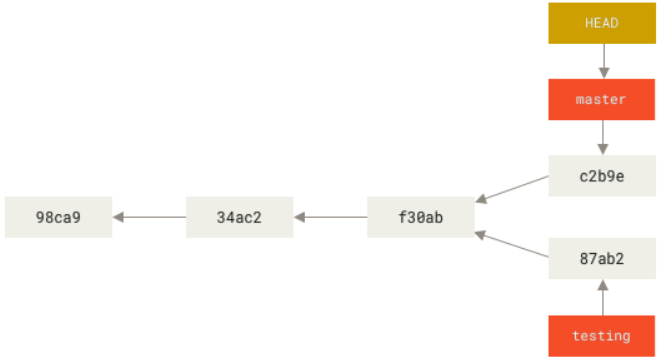
\includegraphics[width=0.475\textwidth]{images/git_branching}
	\caption{Git branching model, two branches exist one called master and one called testing~\cite{pro_git}.}
\label{fig:git_branching}
\end{figure}

Commits contain more information than just changes to file contents---they also include information about who authored the commit and who last applied it (for example, when a commit is imported from a patch file or when the commit is part of a rebase) known as the author and committer respectively.
The field of mining software repositories (MSR) attempts to analyze the contents of software repositories to obtain useful information about a software project~\cite{road_ahead_for_msr}.

Commits are ordered according to their parents.
We can traverse the history of the repository by reversing the changes applied by each commit.
Starting at \codeword{c2b9e} in \autoref{fig:git_branching} the history would contain \codeword{f30ab}, \codeword{34ac2} and \codeword{98ca9} in order of the most recent commits.
Therefore, we can define a window of commits as a subset of all commits in the repository which form a continuous history.
We will traverse this window of commits, and we can apply filter operations to reduce the total amount of commits to be selected based on some metrics (for example files changed, author, time between commits etc.).

Code analysis tools provide various metrics which are used to assess the quality of software code.
Such metrics which may be used include test coverage, and security vulnerabilities.
Tools which do not execute the code but instead analyse the code by reading it are called static code analysis tools.
One common type of static code analysis is static application security testing (SAST).
A SAST tool such a Snyk Code or SonarQube Security Analysis will analyze the code to detect common security vulnerabilities such as the use of known weak hashing or encryption algorithms, or known vulnerable dependency versions~\cite{scat}.
One common limitation of these tools, however, is that they only perform analysis on one version of the software---that is, the version of the software they are provided as they are executed.
Previous versions of the software could still be in use and if a new vulnerability is discovered in a dependency used by older versions of the software, but that version of the dependency is not used by the most recent version of the software, the SAST tool will not identify this vulnerability.
This is a very likely scenario for SAST tools which are constantly updating their vulnerability databases as new vulnerabilities are found and so a scenario where a vulnerability was not known at the time of release but has since been discovered is very likely.

Another example of a code analysis tool is unit test coverage.
This type of tool will run tests written for the software and calculate the percentage of the program tested---often the total lines tested is used but other metrics such as branches taken are also used.
As with SAST tools, code coverage tools only perform analysis on the single version of the software provided to them.
A tool which can perform analysis across different historic versions of the software would enable time series data to be produced to understand how code coverage changes over time.

Iterating through each version of a project sequentially and running analysis can be slow (the Linux repository for example has over 1.3m commits as of Dec 2022 and if each commit only took 1 second to be checked out and analysed it would still take 15 days to go through every commit~\cite{linux_git}).
As each analysis is independent of one another, this problem is very suitable for parallelization which can be used to significantly speed up analysis.
Each process could use an isolated environment to avoid overwriting output from other processes.

Given the common limitation of SCA tools performing analysis on just one version of a software project, a tool called GitSlice has been developed to perform analysis on many versions of a project.
GitSlice allows for a configurable subset of commits in a repository to be selected for analysis using any arbitrary third-party SCA tool.
The analysis tool is run in an isolated environment in parallel and provided with different versions of the project.
The output from this tool is then saved as separate files to an output directory, the names of these files and the output directory are also configurable.
This output can then be used to produce time series data or for further analysis to be performed.
